\documentclass[a4paper, 11pt]{article}

\usepackage{fullpage}
\usepackage[svgnames,x11names]{xcolor}
\usepackage{hyperref}
\hypersetup{
  breaklinks,
  colorlinks,
  linkcolor={blue!50!black},
  citecolor={blue!50!black},
  urlcolor={blue!50!black}
}
\usepackage{amsthm}
\usepackage[numbers,sort&compress]{natbib}
\usepackage{listings}
\usepackage{xspace}
\usepackage{graphicx}

\newcommand*{\Modone}{Bank\xspace}%
\newcommand*{\modone}{bank\xspace}%
\newcommand*{\Modtwo}{Shopping Mall\xspace}%
\newcommand*{\modtwo}{shopping mall\xspace}%
\newcommand*{\Modthree}{Network Operator\xspace}%
\newcommand*{\modthree}{network operator\xspace}%
\newcommand*{\Modfour}{Notary\xspace}%
\newcommand*{\modfour}{notary\xspace}%
\newcommand*{\Modfive}{Government\xspace}%
\newcommand*{\modfive}{government\xspace}%

\theoremstyle{definition}
\newtheorem{exercise}{Exercise}

\begin{document}
%%% Header starts
\noindent{\large\textbf{IS-521 Activity}\hfill
                \textbf{Team-based Software Engineering (part 2)} \\
         {\phantom{} \hfill Due Date: May 29, 2017 (before class)} \\
%%% Header ends

\section{Activity Overview}

In this activity, each team is given a server VM. Your goal is to
setup the environment for running all the services developed in the
previous activity. Each VM has total 8 NICs (from eth0 to eth7). You
can ignore the eth0, but other NICs are bind to a specific IP address,
which is described in \S\ref{ipaddrs}. Your final submission should be
a single installation script that sets up your server without any user
intervention.

\section{Deliverable}

We expect a single script (in any language) that installs every
component of your server including bank, notary, visualizer, etc. Each
team leader should demonstrate their server settings in the class.
%
Each team leader can create a private repository in GitHub to store
the script.

When you do this activity, you do have a root access on the VM,
because you need to install required packages and change system
configurations. However, in the final CTF, we are not giving you a
root access, since we do not want you to patch (modify) your service
binaries during the CTF. Remember, you can only use Snort for defenses
in the final CTF.

As an example, you may want to create a BASH script that starts with
the following commands:
\begin{verbatim}
#!/bin/bash
# Clone all the repos
git clone git@github.com:KAIST-IS521/TeamOne.git TeamOne
git clone git@github.com:KAIST-IS521/TeamTwo.git TeamTwo
# omitted ...
\end{verbatim}

\section{List of VMs} \label{ipaddrs}

We provide a single VM for each team. We will \emph{not} disclose the
IP address here, but will let you know in the class. Below is the list
of VMs.
%
\begin{enumerate}
%
  \item Team 1's VM: Port 10000
  \item Team 2's VM: Port 20000
  \item Team 3's VM: Port 30000
  \item Team 4's VM: Port 40000
  \item Team 5's VM: Port 50000
%
\end{enumerate}

\section{Setup}

\subsection{Network}

\begin{figure}[t]
  \centering
  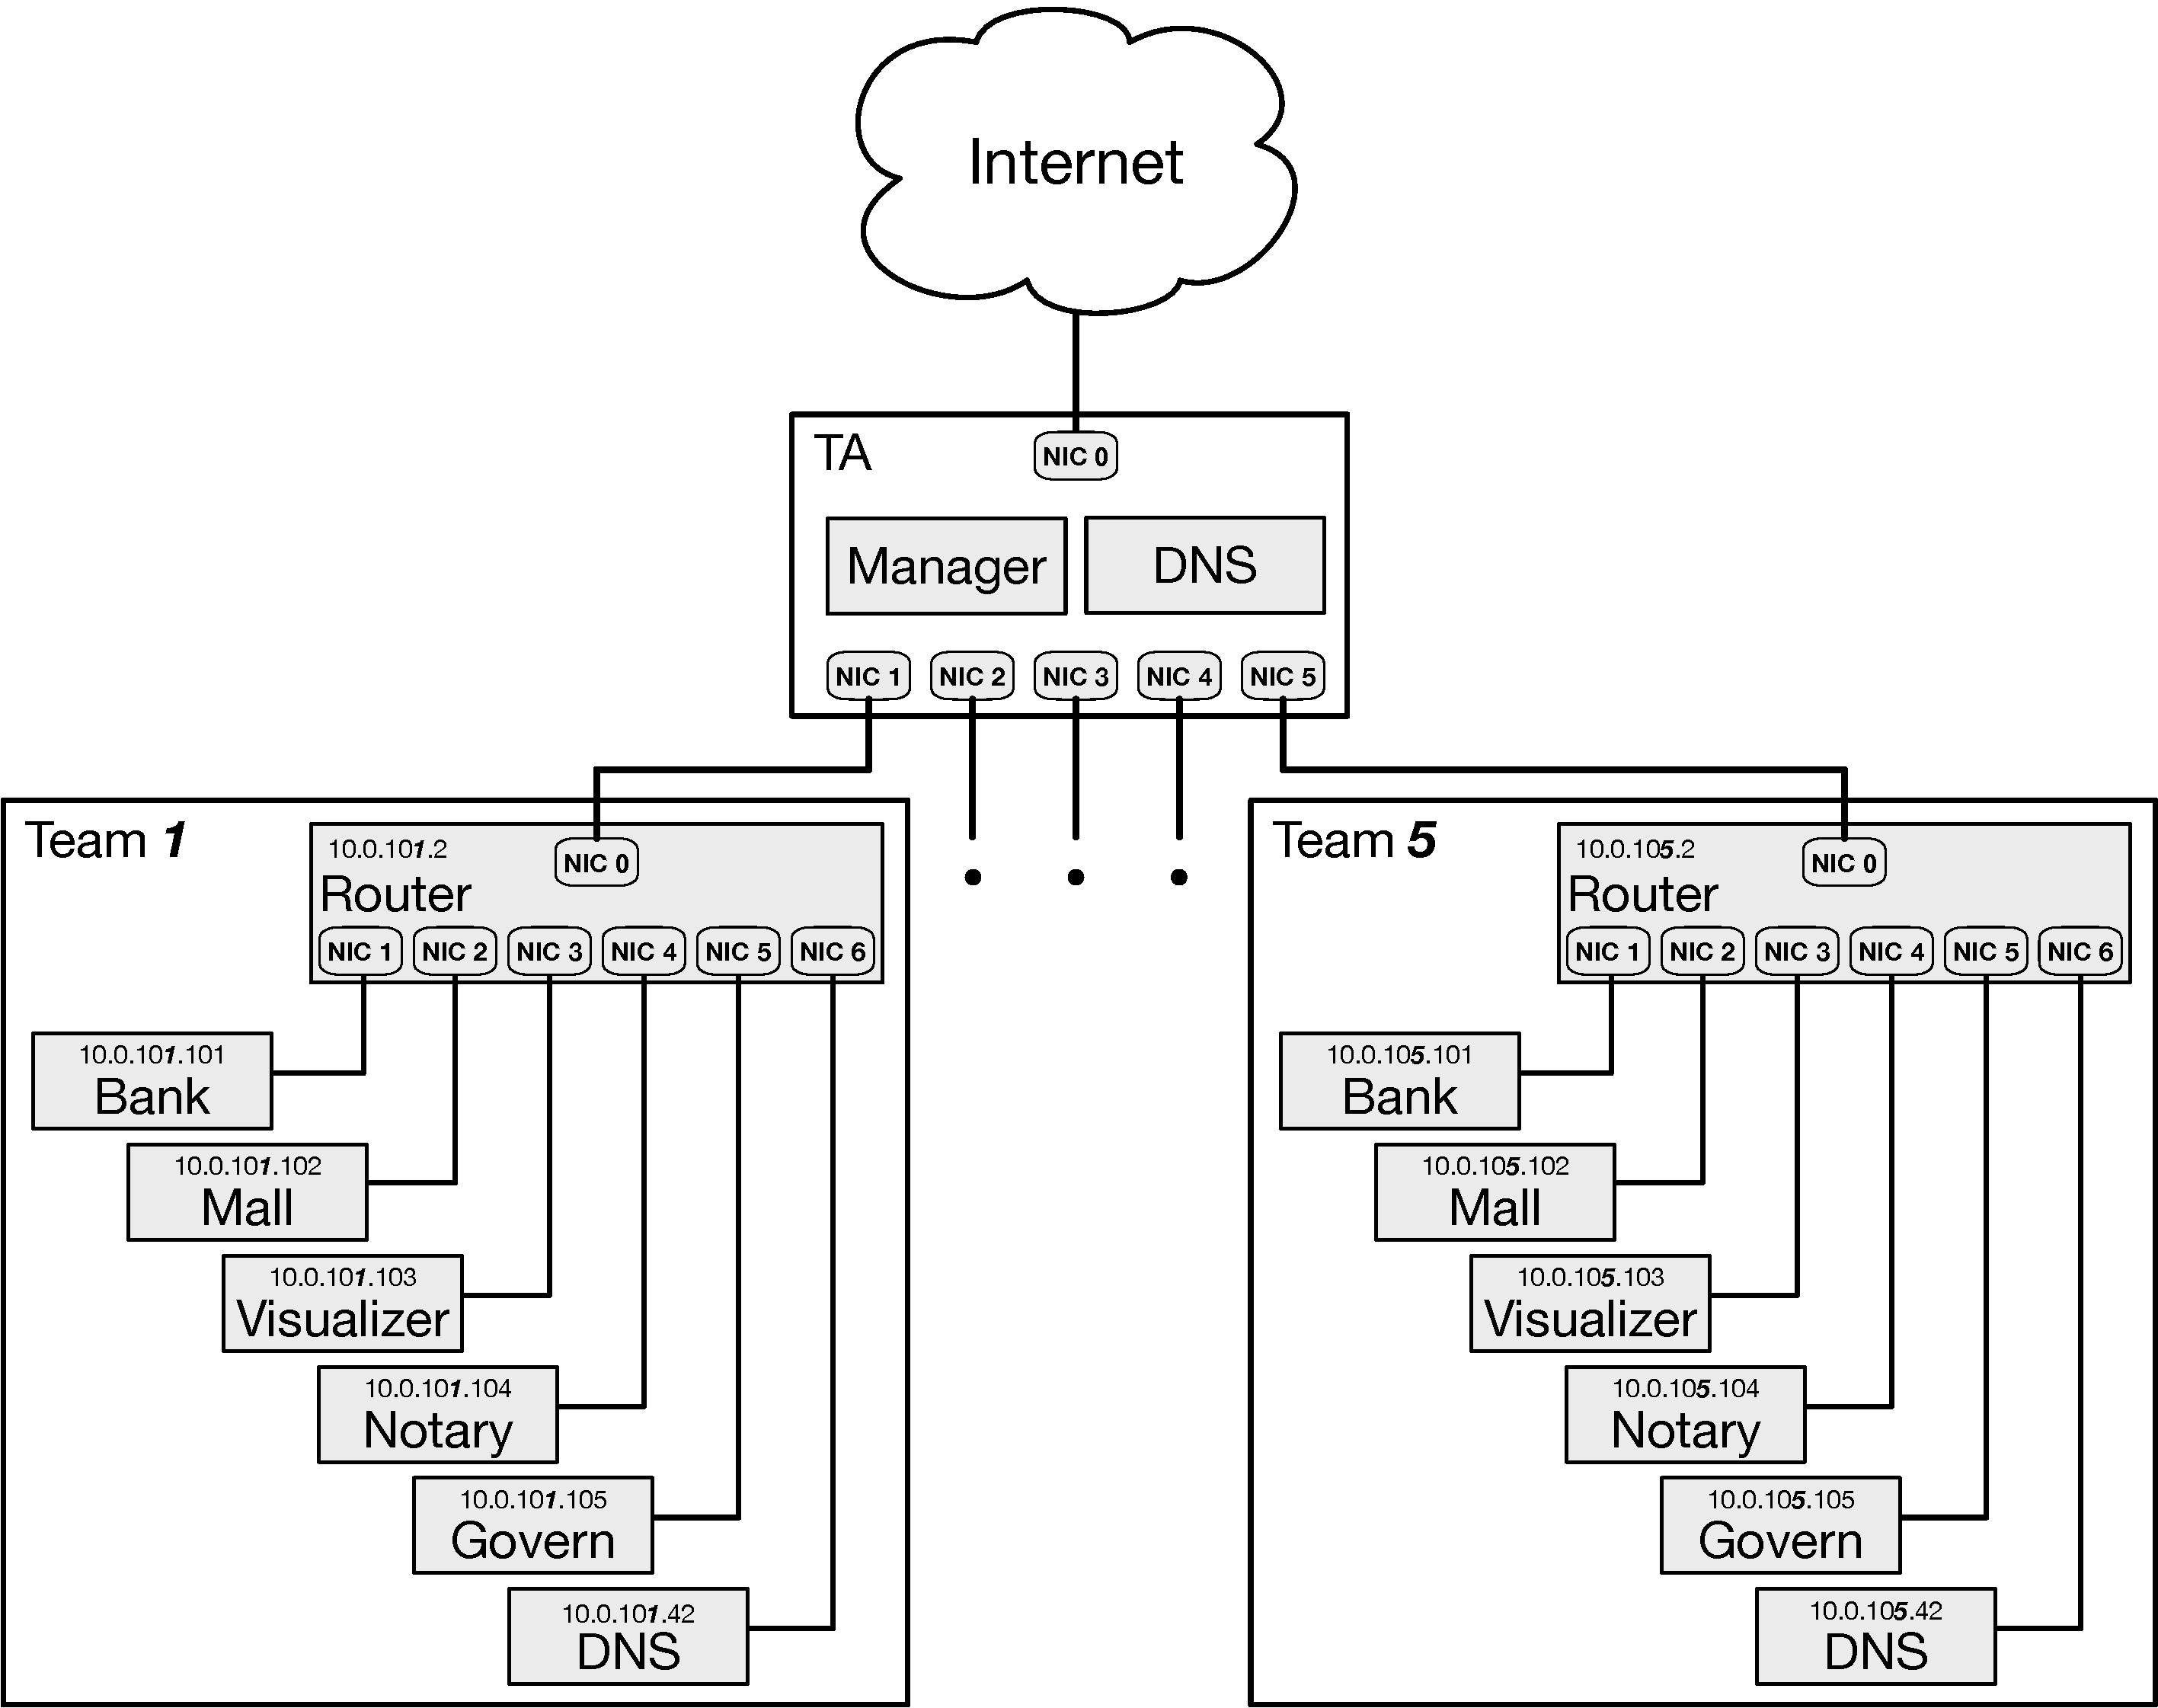
\includegraphics[width=\linewidth]{figs/network}
  \caption{CTF Network.}
  \label{fig:net}
\end{figure}

Figure~\ref{fig:net} presents our network settings. Each team has its
own private network, and runs every service developed in the previous
activity. Each team can talk to each other only via the TA's router.
The TA's router has 5 NICs installed that connect to each team's
router. IP addresses of each component in the network follows the
convention described below.

\begin{enumerate}
%
  \item Team \texttt{X}'s router is at \texttt{10.0.10X.2}.
%
  \item Team \texttt{X}'s bank service is at \texttt{10.0.10X.101}.
%
  \item Team \texttt{X}'s shopping mall service is at
    \texttt{10.0.10X.102}.
%
  \item Team \texttt{X}'s network operator service is at
    \texttt{10.0.10X.103}.
%
  \item Team \texttt{X}'s notary service is at \texttt{10.0.10X.104}.
%
  \item Team \texttt{X}'s government service is at \texttt{10.0.10X.105}.
%
  \item Team \texttt{X}'s DNS cache is at \texttt{10.0.10X.42}.
%
\end{enumerate}

\subsection{Sandboxing}

For security reason, you need to sandbox each service in a docker
image~\cite{docker}. If you are new to docker, their
tutorial~\cite{dockertutorial} is a good starting point.

\subsection{DNS}

Every service (i.e., docker) in your network should use your local DNS
cache located at \texttt{10.0.10X.42}. This DNS cache should be set up
with a program called \texttt{dnsmasq}.

Your DNS cache should use \texttt{192.168.127.15} as its primary DNS
server. Any service should be accessible via teams' domain names. For
example, we should be able to access the team1's banking service with
\texttt{bank.team1}.
\begin{enumerate}
  \item Team \texttt{X}'s bank service: \texttt{bank.teamX}.
  \item Team \texttt{X}'s shopping mall service: \texttt{mall.teamX}.
  \item Team \texttt{X}'s government service: \texttt{gov.teamX}.
  \item Team \texttt{X}'s notary service: \texttt{notary.teamX}.
  \item Team \texttt{X}'s network operator service: \texttt{viz.teamX}.
\end{enumerate}


\section{Grading}

Your team will get full points if your server works properly, i.e.,
all the services pass the SLA checks after running your installation
script.

We also recommend you to submit pull requests (PRs) to other teams.
Again, we are going to give an individual extra points for a PR. As
always, we will \emph{not} give extra points for every PR.

\bibliography{references}
\bibliographystyle{plainnat}

\end{document}
